% Options for packages loaded elsewhere
\PassOptionsToPackage{unicode}{hyperref}
\PassOptionsToPackage{hyphens}{url}
%
\documentclass[
  ignorenonframetext,
  aspectratio=169,
  russian,
]{beamer}
\usepackage{pgfpages}
\setbeamertemplate{caption}[numbered]
\setbeamertemplate{caption label separator}{: }
\setbeamercolor{caption name}{fg=normal text.fg}
\beamertemplatenavigationsymbolshorizontal
% Prevent slide breaks in the middle of a paragraph
\widowpenalties 1 10000
\raggedbottom
\setbeamertemplate{part page}{
  \centering
  \begin{beamercolorbox}[sep=16pt,center]{part title}
    \usebeamerfont{part title}\insertpart\par
  \end{beamercolorbox}
}
\setbeamertemplate{section page}{
  \centering
  \begin{beamercolorbox}[sep=12pt,center]{section title}
    \usebeamerfont{section title}\insertsection\par
  \end{beamercolorbox}
}
\setbeamertemplate{subsection page}{
  \centering
  \begin{beamercolorbox}[sep=8pt,center]{subsection title}
    \usebeamerfont{subsection title}\insertsubsection\par
  \end{beamercolorbox}
}
\AtBeginPart{
  \frame{\partpage}
}
\AtBeginSection{
  \ifbibliography
  \else
    \frame{\sectionpage}
  \fi
}
\AtBeginSubsection{
  \frame{\subsectionpage}
}

\usepackage{amsmath,amssymb}
\usepackage{iftex}
\ifPDFTeX
  \usepackage[T1]{fontenc}
  \usepackage[utf8]{inputenc}
  \usepackage{textcomp} % provide euro and other symbols
\else % if luatex or xetex
  \usepackage{unicode-math}
  \defaultfontfeatures{Scale=MatchLowercase}
  \defaultfontfeatures[\rmfamily]{Ligatures=TeX,Scale=1}
\fi
\usepackage{lmodern}
\ifPDFTeX\else  
    % xetex/luatex font selection
\fi
% Use upquote if available, for straight quotes in verbatim environments
\IfFileExists{upquote.sty}{\usepackage{upquote}}{}
\IfFileExists{microtype.sty}{% use microtype if available
  \usepackage[]{microtype}
  \UseMicrotypeSet[protrusion]{basicmath} % disable protrusion for tt fonts
}{}
\usepackage{xcolor}
\newif\ifbibliography
\setlength{\emergencystretch}{3em} % prevent overfull lines
\setcounter{secnumdepth}{-\maxdimen} % remove section numbering


\providecommand{\tightlist}{%
  \setlength{\itemsep}{0pt}\setlength{\parskip}{0pt}}\usepackage{longtable,booktabs,array}
\usepackage{calc} % for calculating minipage widths
\usepackage{caption}
% Make caption package work with longtable
\makeatletter
\def\fnum@table{\tablename~\thetable}
\makeatother
\usepackage{graphicx}
\makeatletter
\newsavebox\pandoc@box
\newcommand*\pandocbounded[1]{% scales image to fit in text height/width
  \sbox\pandoc@box{#1}%
  \Gscale@div\@tempa{\textheight}{\dimexpr\ht\pandoc@box+\dp\pandoc@box\relax}%
  \Gscale@div\@tempb{\linewidth}{\wd\pandoc@box}%
  \ifdim\@tempb\p@<\@tempa\p@\let\@tempa\@tempb\fi% select the smaller of both
  \ifdim\@tempa\p@<\p@\scalebox{\@tempa}{\usebox\pandoc@box}%
  \else\usebox{\pandoc@box}%
  \fi%
}
% Set default figure placement to htbp
\def\fps@figure{htbp}
\makeatother

\IfFileExists{plex-otf.sty}{
  %% Full TeXlive
  % \usepackage[%
  %   % math,
  %   RM={Scale=0.94},SS={Scale=0.94},SScon={Scale=0.94},TT={Scale=MatchLowercase,FakeStretch=0.9},DefaultFeatures={Ligatures=Common}
  % ]{plex-otf}
}{
  %% TinyTeX
  \usepackage{libertine}
}

%%% Load theme
% https://deic.uab.cat/~iblanes/beamer_gallery/
\IfFileExists{beamerthemegotham.sty}{
  %% Full TeXlive
  \usetheme{gotham}
  \gothamset{
    numbering=totalpagenumber,
    parttocframe default=off,
    sectiontocframe default=off,
    subsectiontocframe default=off,
  }
}{
  %% TinyTeX
  \usetheme{Madrid}
}
\makeatletter
\@ifpackageloaded{caption}{}{\usepackage{caption}}
\AtBeginDocument{%
\ifdefined\contentsname
  \renewcommand*\contentsname{Содержание}
\else
  \newcommand\contentsname{Содержание}
\fi
\ifdefined\listfigurename
  \renewcommand*\listfigurename{Список иллюстраций}
\else
  \newcommand\listfigurename{Список иллюстраций}
\fi
\ifdefined\listtablename
  \renewcommand*\listtablename{Список таблиц}
\else
  \newcommand\listtablename{Список таблиц}
\fi
\ifdefined\figurename
  \renewcommand*\figurename{Рисунок}
\else
  \newcommand\figurename{Рисунок}
\fi
\ifdefined\tablename
  \renewcommand*\tablename{Таблица}
\else
  \newcommand\tablename{Таблица}
\fi
}
\@ifpackageloaded{float}{}{\usepackage{float}}
\floatstyle{ruled}
\@ifundefined{c@chapter}{\newfloat{codelisting}{h}{lop}}{\newfloat{codelisting}{h}{lop}[chapter]}
\floatname{codelisting}{Список}
\newcommand*\listoflistings{\listof{codelisting}{Листинги}}
\makeatother
\makeatletter
\makeatother
\makeatletter
\@ifpackageloaded{caption}{}{\usepackage{caption}}
\@ifpackageloaded{subcaption}{}{\usepackage{subcaption}}
\makeatother

\usepackage{polyglossia}
\setmainfont{DejaVu Serif}
\setsansfont{DejaVu Sans}
\setmonofont{DejaVu Sans Mono}
\newfontfamily\cyrillicfont{DejaVu Serif}
\newfontfamily\cyrillicfontsf{DejaVu Sans}
\newfontfamily\cyrillicfonttt{DejaVu Sans Mono}
\setdefaultlanguage{russian}
\setotherlanguage{english}
\usepackage{csquotes}
\usepackage{bookmark}

\IfFileExists{xurl.sty}{\usepackage{xurl}}{} % add URL line breaks if available
\urlstyle{same} % disable monospaced font for URLs
\hypersetup{
  pdftitle={Лабораторная работа №7},
  pdfauthor={Курилко-Рюмин Евгений Михайлович},
  pdflang={ru-RU},
  hidelinks,
  pdfcreator={LaTeX via pandoc}}


\title{Лабораторная работа №7}
\subtitle{Дискретно-событийное моделирование}
\author{Курилко-Рюмин Евгений Михайлович}
\date{2026-05-16}

\begin{document}
\frame{\titlepage}

\renewcommand*\contentsname{Содержание}
\begin{frame}[allowframebreaks]
  \frametitle{Содержание}
  \setcounter{tocdepth}{1}
  \tableofcontents
\end{frame}

\section{Цель
работы}\label{ux446ux435ux43bux44c-ux440ux430ux431ux43eux442ux44b}

\begin{frame}[fragile]{Цель работы}
\begin{itemize}[<+->]
\tightlist
\item
  Реализовать модели \texttt{M/M/c} и Росса средствами
  дискретно-событийного моделирования
\item
  Подготовить воспроизводимый проект \texttt{DrWatson}
\item
  Построить графики и сравнить имитацию с аналитикой
\end{itemize}
\end{frame}

\section{Задание}\label{ux437ux430ux434ux430ux43dux438ux435}

\begin{frame}[fragile]{Задание}
\begin{itemize}[<+->]
\tightlist
\item
  Выполнить базовый код модели \texttt{M/M/c}
\item
  Добавить графики для многоканальной очереди
\item
  Расширить модель Росса до нескольких ремонтников
\item
  Провести серию прогонов при разном числе машин
\item
  Оценить загрузку ремонтников и длину очереди на ремонт
\item
  Подготовить \texttt{literate}, \texttt{ipynb} и \texttt{qmd}
\end{itemize}
\end{frame}

\section{Архитектура
проекта}\label{ux430ux440ux445ux438ux442ux435ux43aux442ux443ux440ux430-ux43fux440ux43eux435ux43aux442ux430}

\begin{frame}[fragile]{Архитектура проекта}
\begin{itemize}[<+->]
\tightlist
\item
  \texttt{src/DiscreteEventLab07Core.jl} --- модуль с двумя моделями
\item
  \texttt{scripts/01\_discrete\_event\_models.jl} --- базовые сценарии
\item
  \texttt{scripts/02\_discrete\_event\_models\_param.jl} ---
  параметрические эксперименты
\item
  \texttt{scripts/generate\_all.jl} --- генерация \texttt{clean},
  \texttt{qmd}, \texttt{ipynb}
\item
  \texttt{test/runtests.jl} --- базовые проверки
\end{itemize}
\end{frame}

\section{Подготовка
окружения}\label{ux43fux43eux434ux433ux43eux442ux43eux432ux43aux430-ux43eux43aux440ux443ux436ux435ux43dux438ux44f}

\begin{frame}[fragile]{Подготовка окружения}
\begin{columns}[T]
\begin{column}{0.5\linewidth}
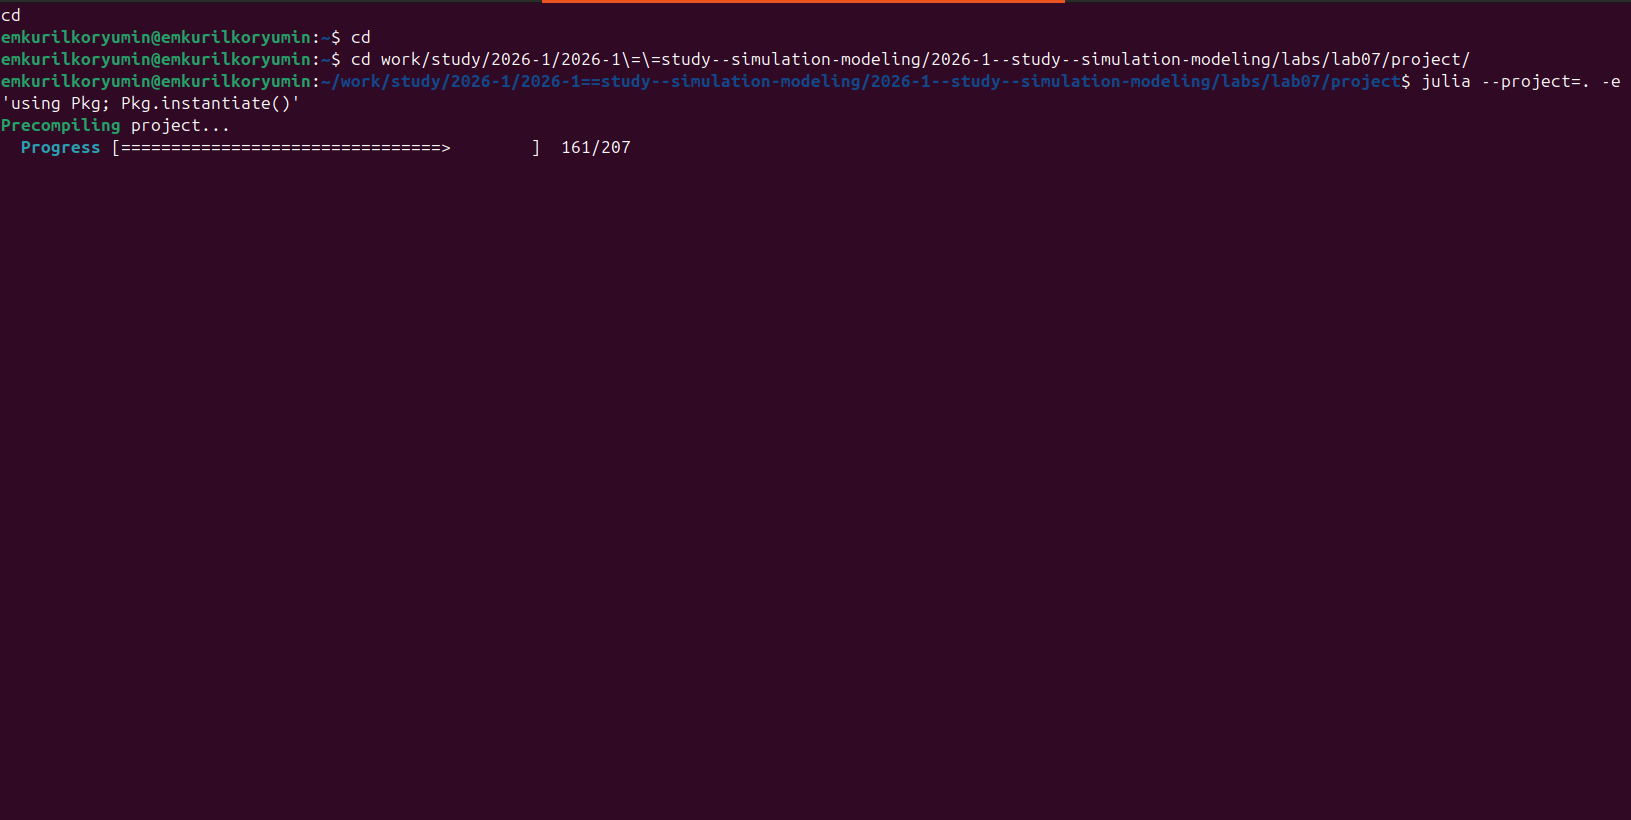
\includegraphics[width=1\linewidth,height=\textheight,keepaspectratio]{image/setup_instantiate_start.png}
\end{column}

\begin{column}{0.5\linewidth}
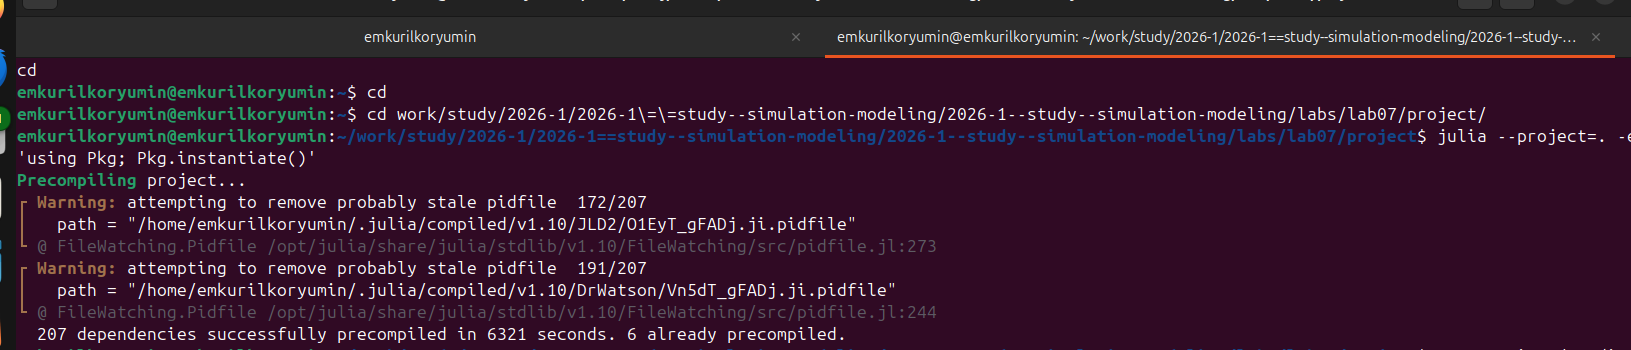
\includegraphics[width=1\linewidth,height=\textheight,keepaspectratio]{image/setup_precompile_done.png}
\end{column}
\end{columns}

\begin{itemize}[<+->]
\tightlist
\item
  Слева показан запуск \texttt{Pkg.instantiate()} в каталоге проекта
\item
  Справа видно успешное завершение предкомпиляции зависимостей
\end{itemize}
\end{frame}

\section{\texorpdfstring{Модель
\texttt{M/M/c}}{Модель M/M/c}}\label{ux43cux43eux434ux435ux43bux44c-mmc}

\begin{frame}[fragile]{Модель \texttt{M/M/c}}
\begin{itemize}[<+->]
\tightlist
\item
  Параметры базового сценария:

  \begin{itemize}[<+->]
  \tightlist
  \item
    \texttt{c\ =\ 2}
  \item
    \texttt{λ\ =\ 0.85}
  \item
    \texttt{μ\ =\ 0.5}
  \item
    \texttt{1500} заявок
  \end{itemize}
\item
  Рассчитывались:

  \begin{itemize}[<+->]
  \tightlist
  \item
    среднее время ожидания
  \item
    среднее время в системе
  \item
    вероятность ожидания
  \item
    средняя длина очереди
  \end{itemize}
\end{itemize}
\end{frame}

\section{Консольные запуски
сценариев}\label{ux43aux43eux43dux441ux43eux43bux44cux43dux44bux435-ux437ux430ux43fux443ux441ux43aux438-ux441ux446ux435ux43dux430ux440ux438ux435ux432}

\begin{frame}[fragile]{Консольные запуски сценариев}
\begin{columns}[T]
\begin{column}{0.5\linewidth}
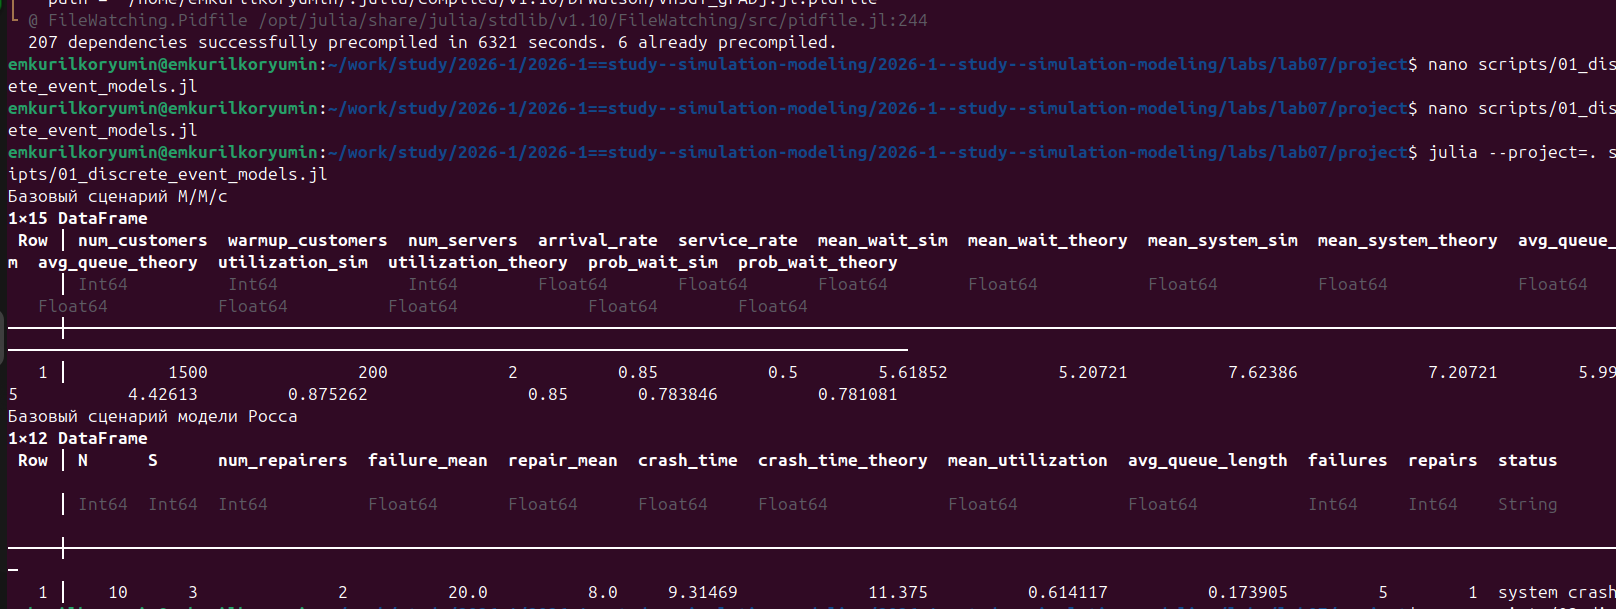
\includegraphics[width=1\linewidth,height=\textheight,keepaspectratio]{image/base_scenarios_console.png}
\end{column}

\begin{column}{0.5\linewidth}
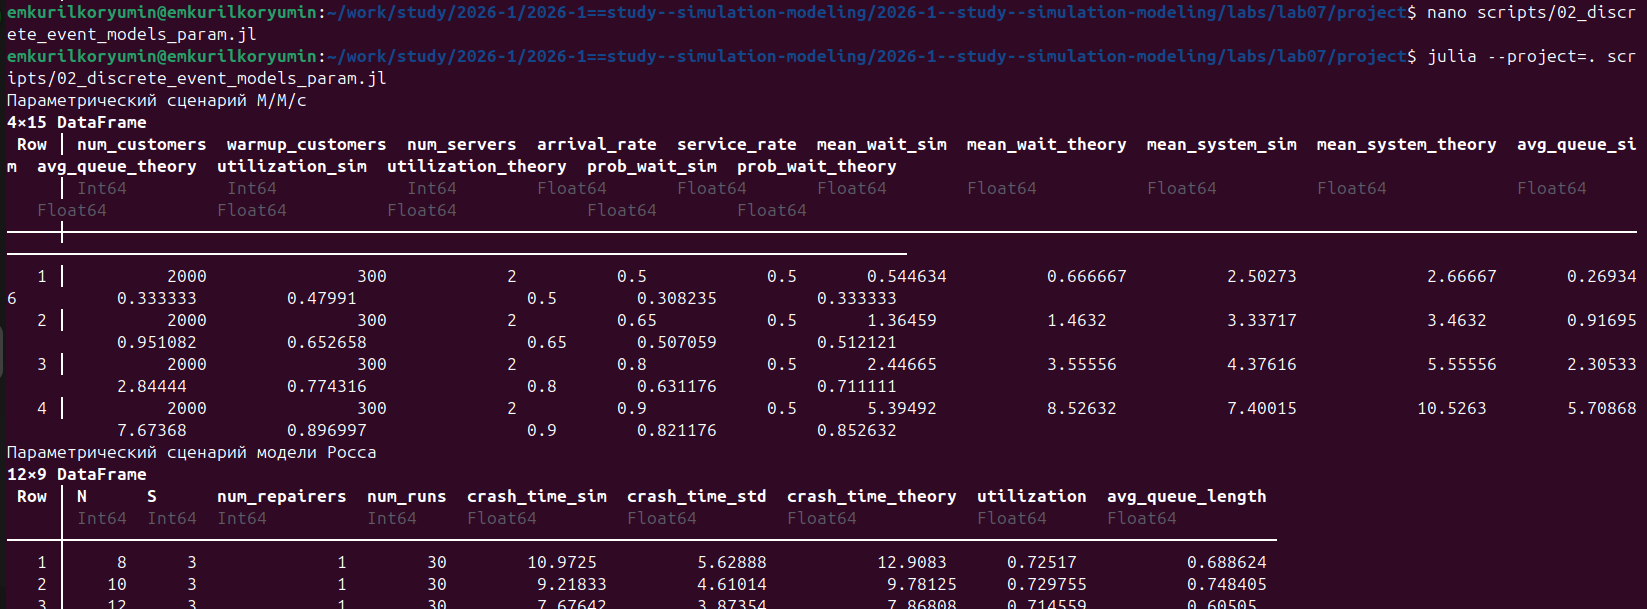
\includegraphics[width=1\linewidth,height=\textheight,keepaspectratio]{image/param_scenarios_console.png}
\end{column}
\end{columns}

\begin{itemize}[<+->]
\tightlist
\item
  Слева: базовый запуск \texttt{M/M/c} и модели Росса
\item
  Справа: параметрический прогон с серией экспериментов
\end{itemize}
\end{frame}

\section{\texorpdfstring{Результаты
\texttt{M/M/c}}{Результаты M/M/c}}\label{ux440ux435ux437ux443ux43bux44cux442ux430ux442ux44b-mmc}

\begin{frame}{Результаты \texttt{M/M/c}}
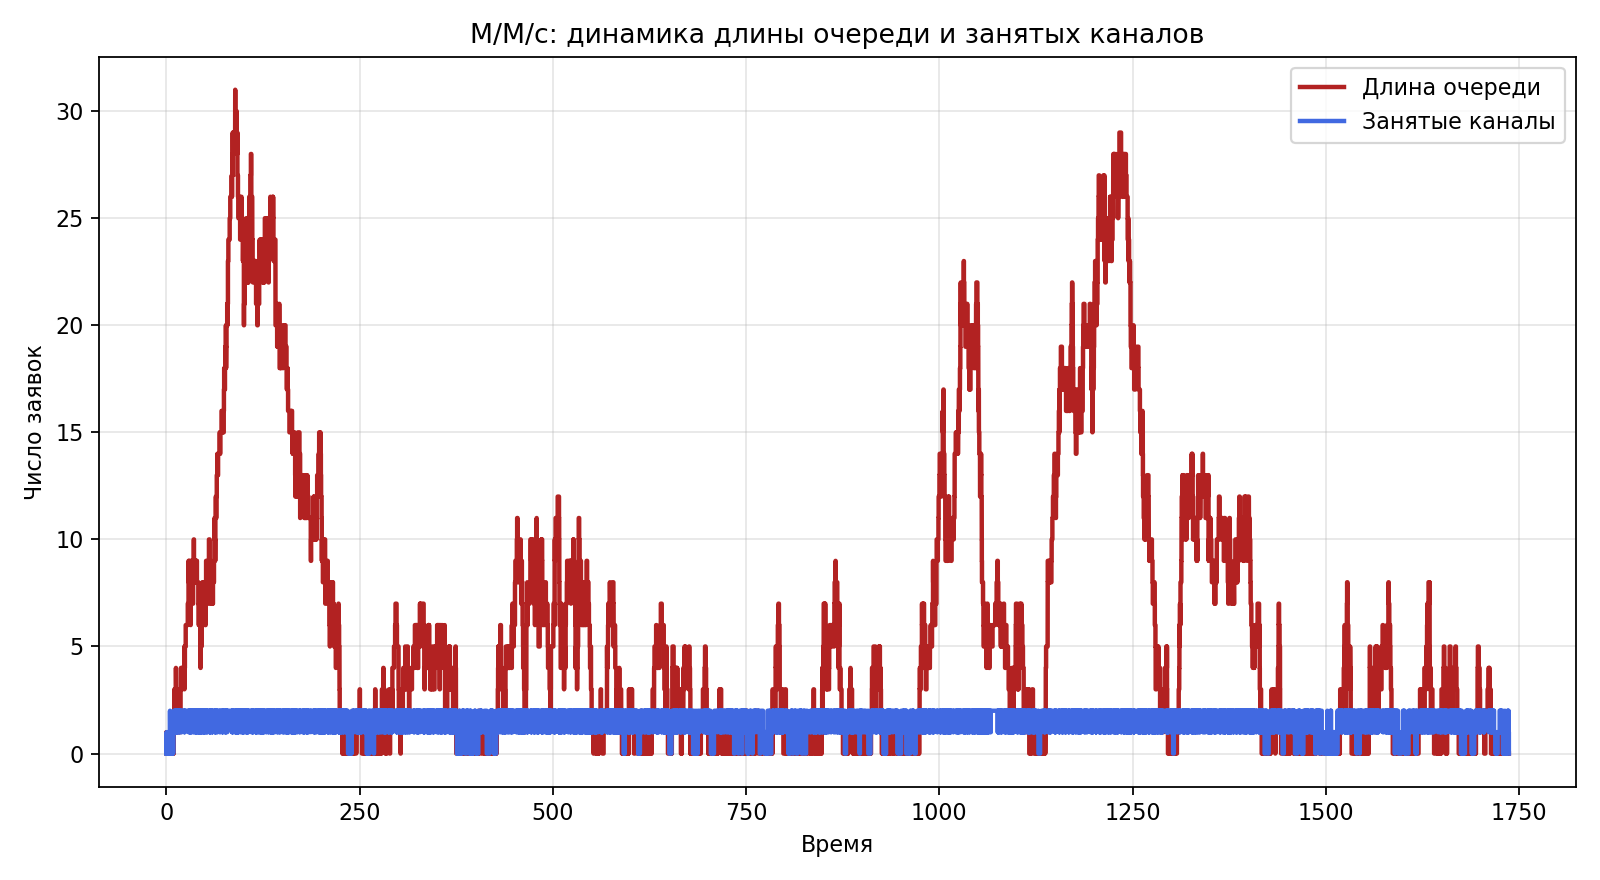
\includegraphics[width=0.9\linewidth,height=\textheight,keepaspectratio]{../project/plots/mmc_queue_timeline.png}

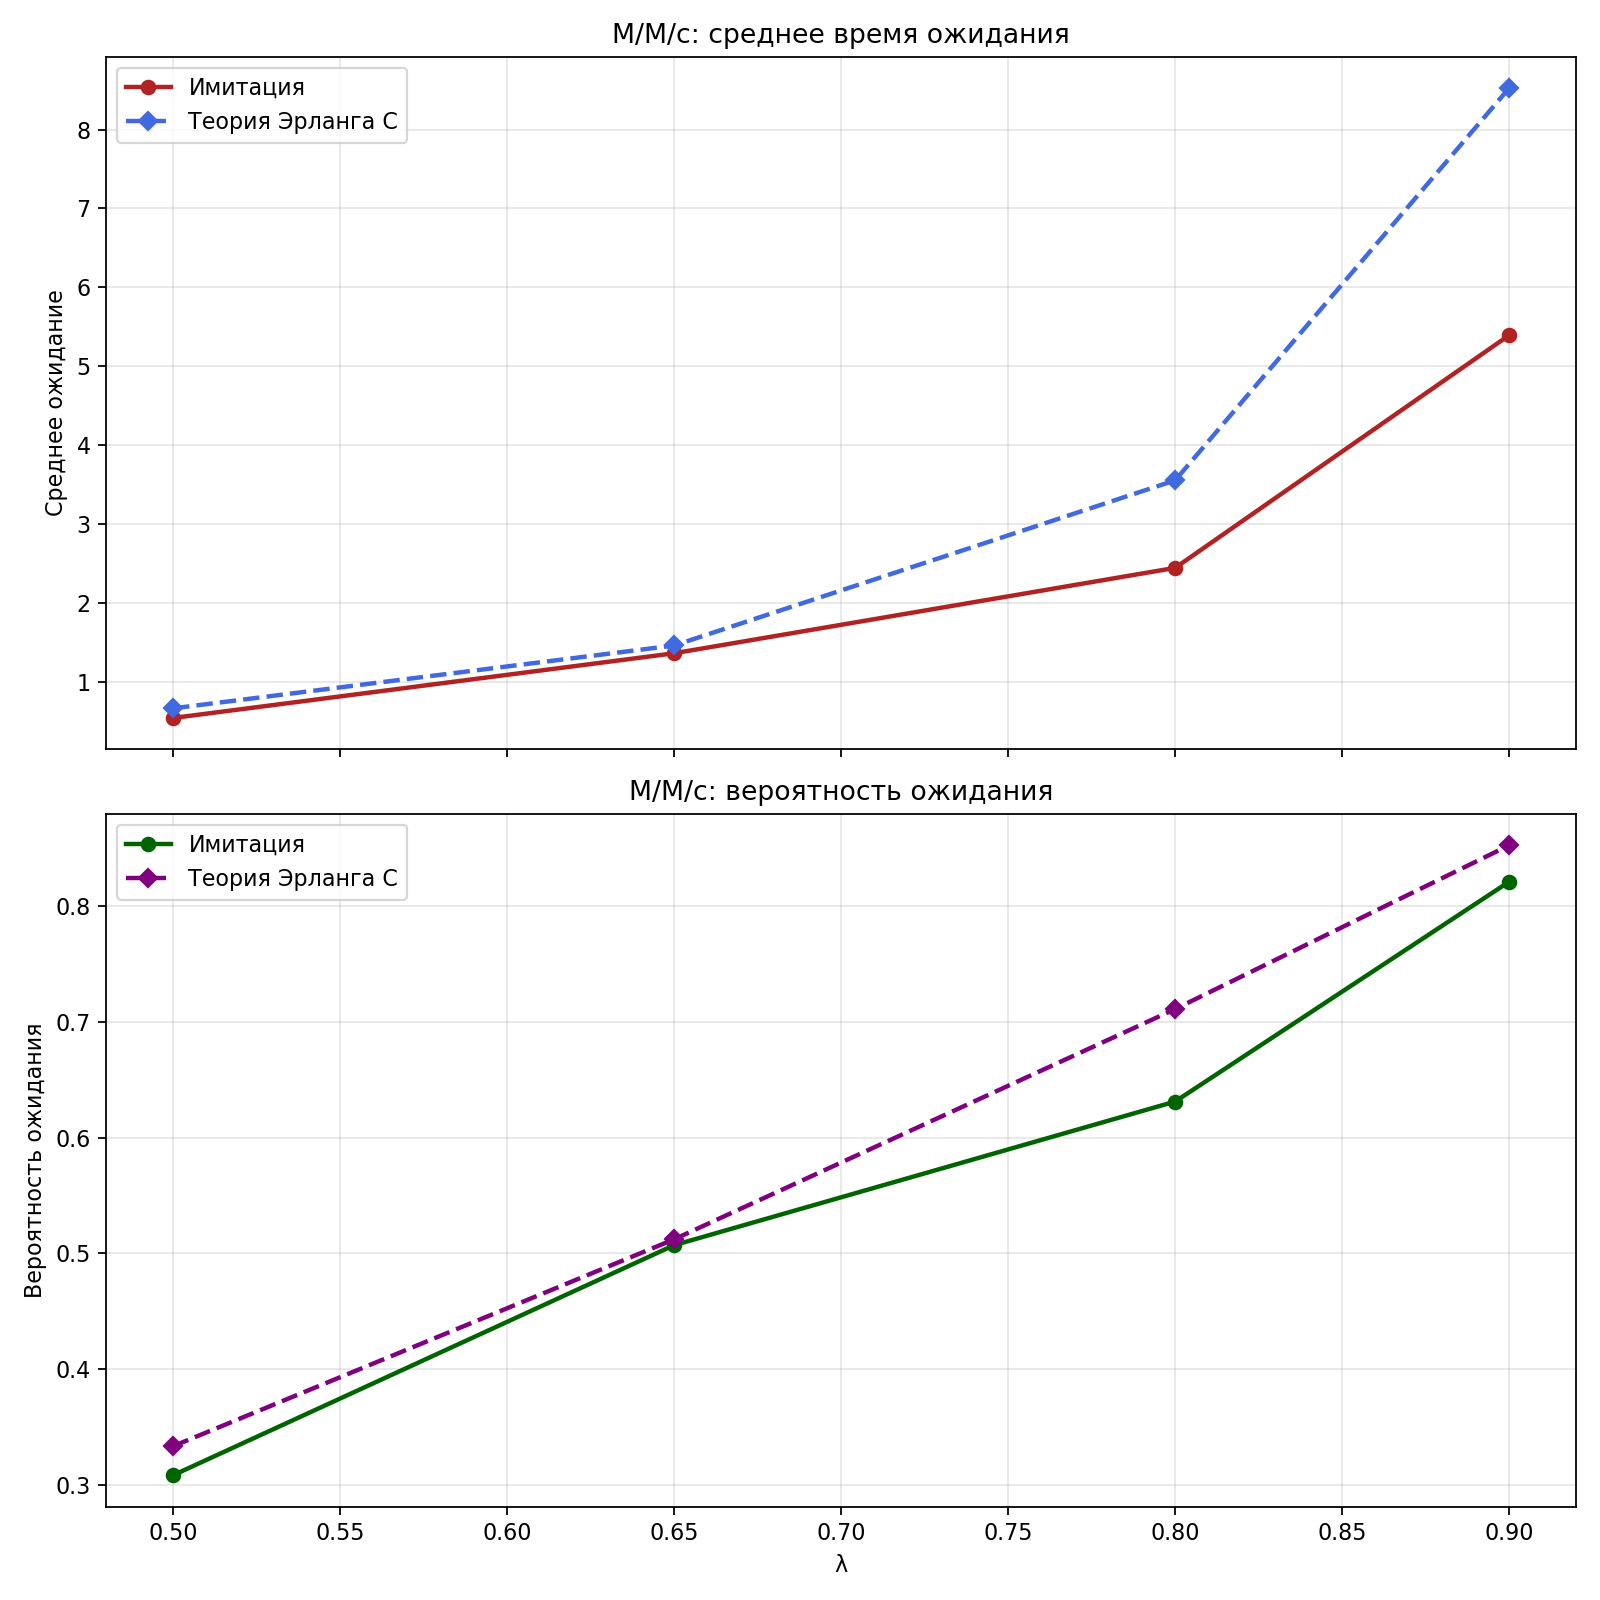
\includegraphics[width=0.9\linewidth,height=\textheight,keepaspectratio]{../project/plots/mmc_wait_vs_lambda.png}
\end{frame}

\section{Модель
Росса}\label{ux43cux43eux434ux435ux43bux44c-ux440ux43eux441ux441ux430}

\begin{frame}[fragile]{Модель Росса}
\begin{itemize}[<+->]
\tightlist
\item
  \texttt{N} основных машин и \texttt{S} резервных машин
\item
  отказавшая машина уходит в ремонт
\item
  при отсутствии резерва система падает
\item
  в лабораторной работе добавлены несколько ремонтников
\item
  дополнительно измерялись:

  \begin{itemize}[<+->]
  \tightlist
  \item
    средняя загрузка ремонтников
  \item
    средняя длина очереди
  \item
    среднее время до отказа
  \end{itemize}
\end{itemize}
\end{frame}

\section{Результаты модели
Росса}\label{ux440ux435ux437ux443ux43bux44cux442ux430ux442ux44b-ux43cux43eux434ux435ux43bux438-ux440ux43eux441ux441ux430}

\begin{frame}{Результаты модели Росса}
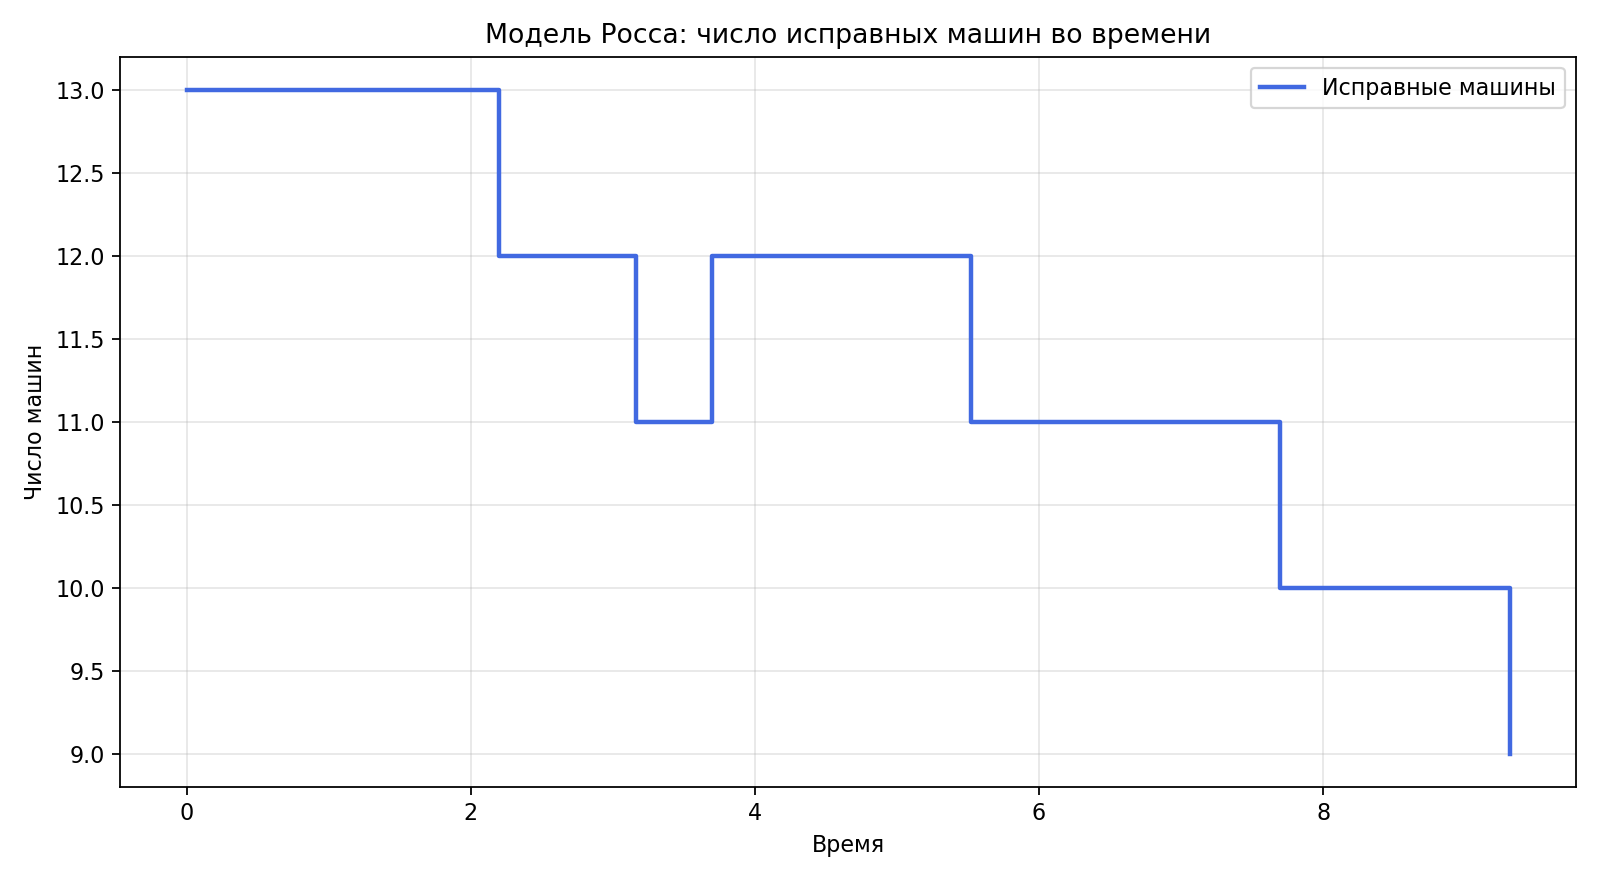
\includegraphics[width=0.9\linewidth,height=\textheight,keepaspectratio]{../project/plots/ross_healthy_timeline.png}

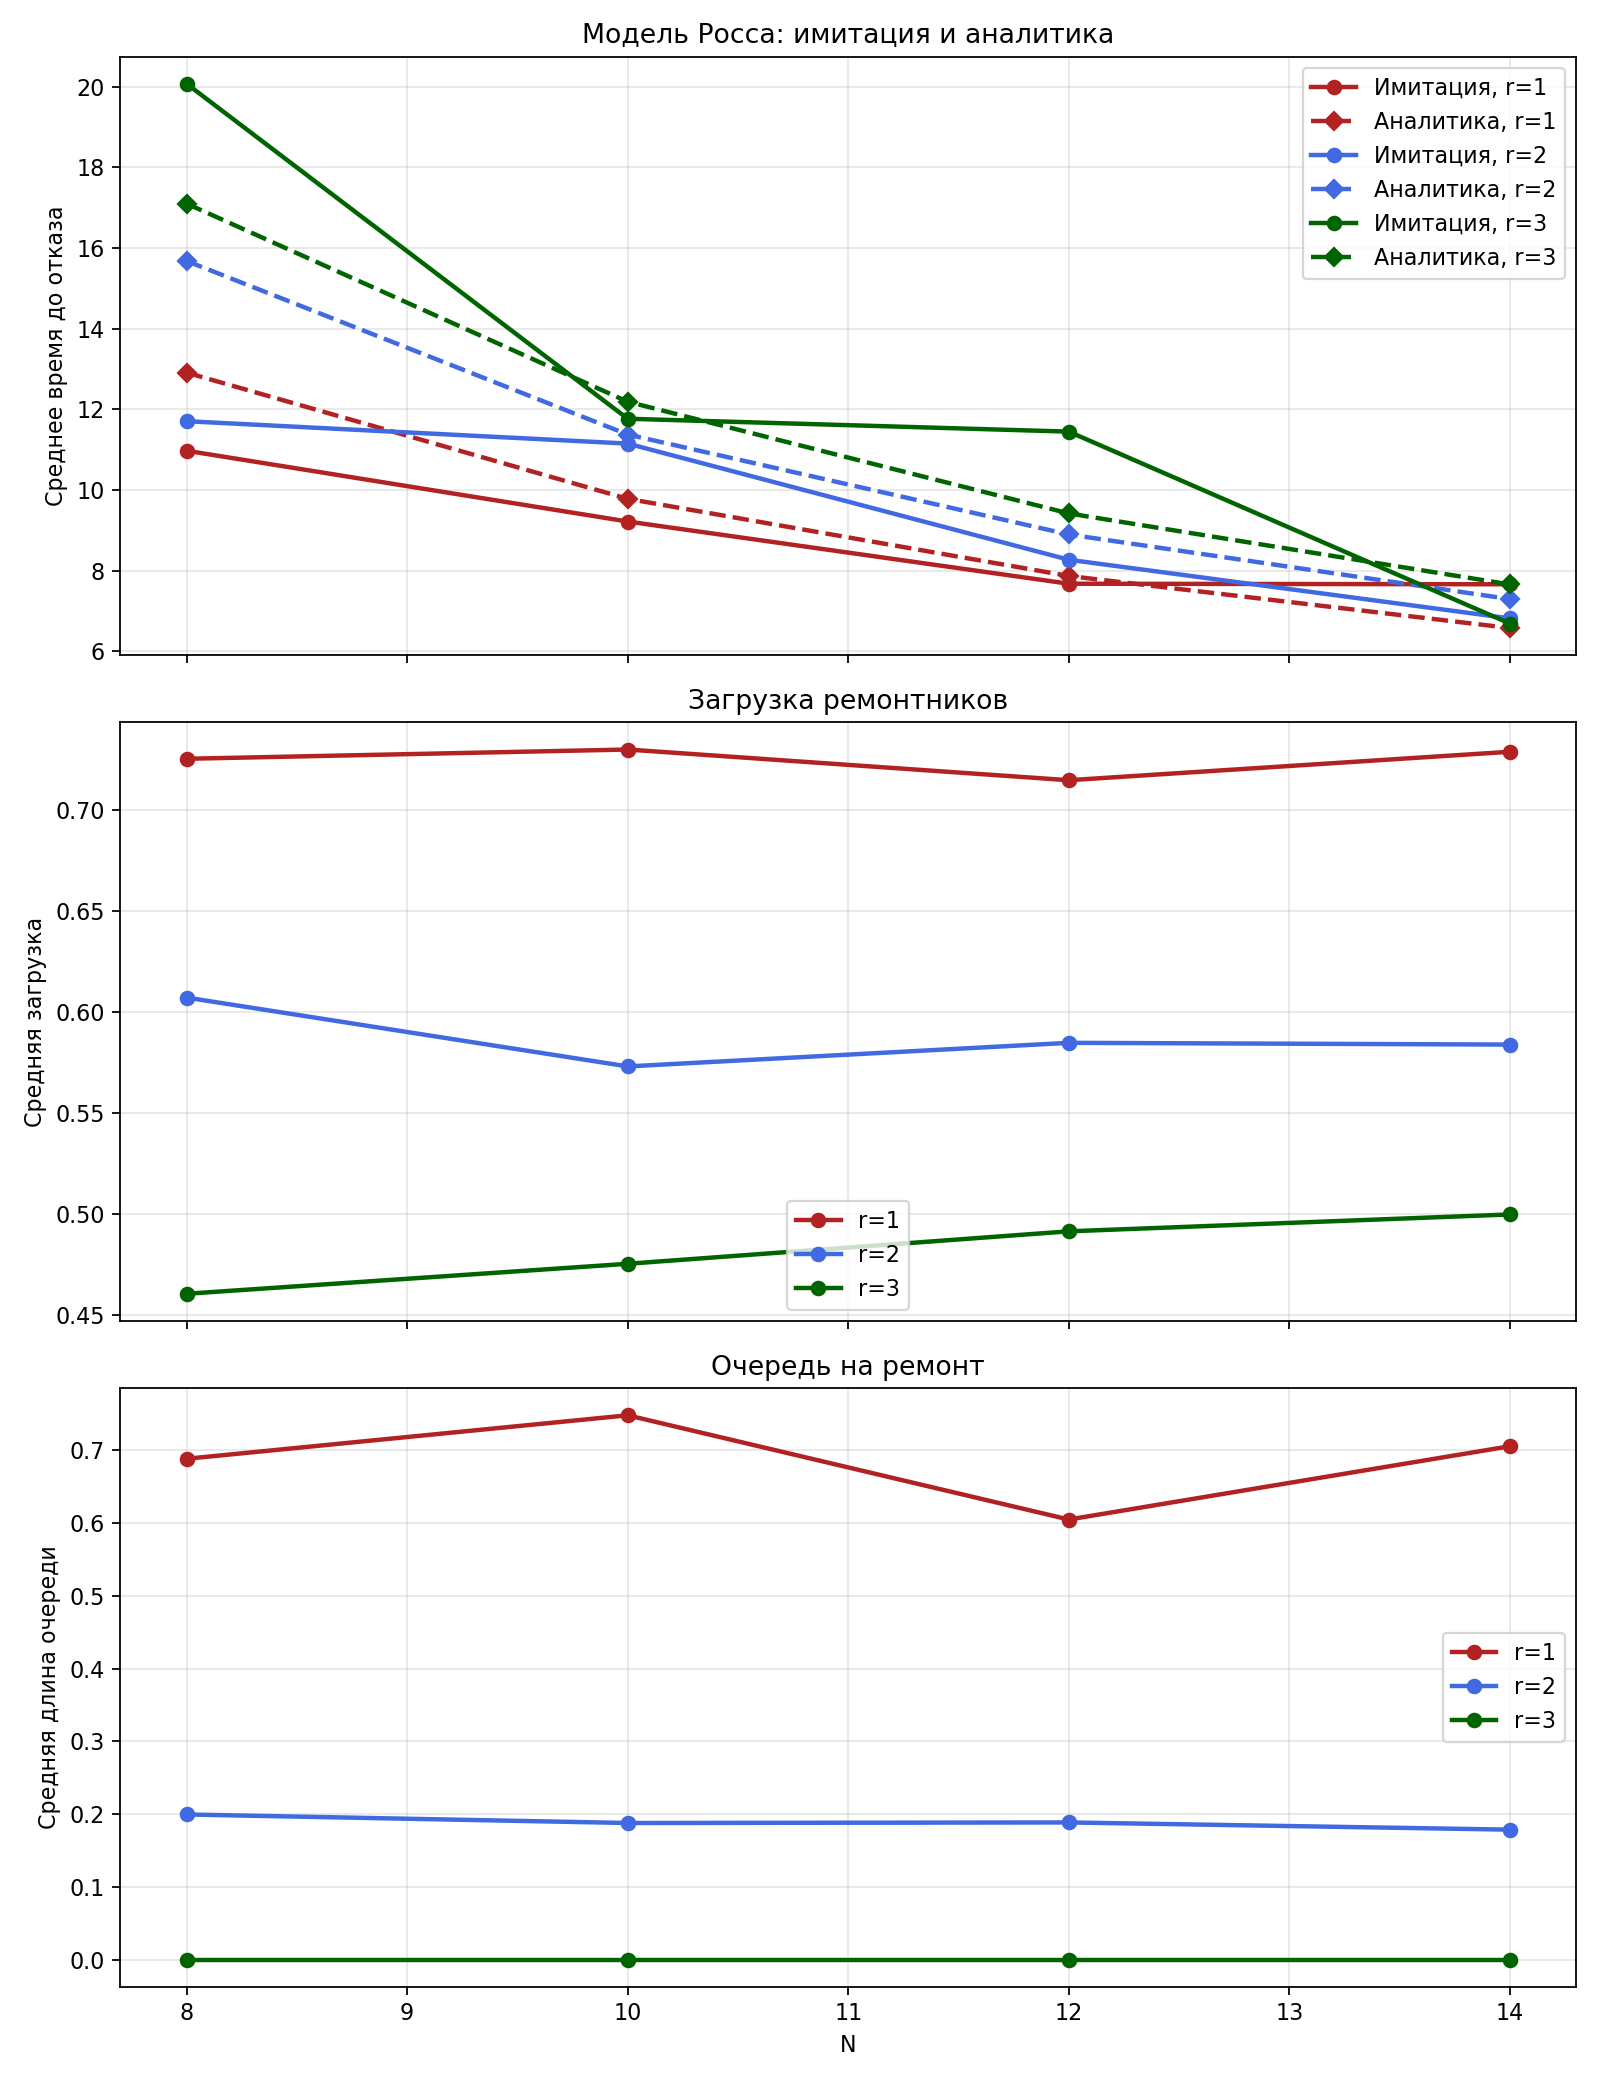
\includegraphics[width=0.9\linewidth,height=\textheight,keepaspectratio]{../project/plots/ross_scan.png}
\end{frame}

\section{Таблицы и генерация
материалов}\label{ux442ux430ux431ux43bux438ux446ux44b-ux438-ux433ux435ux43dux435ux440ux430ux446ux438ux44f-ux43cux430ux442ux435ux440ux438ux430ux43bux43eux432}

\begin{frame}[fragile]{Таблицы и генерация материалов}
\begin{columns}[T]
\begin{column}{0.5\linewidth}
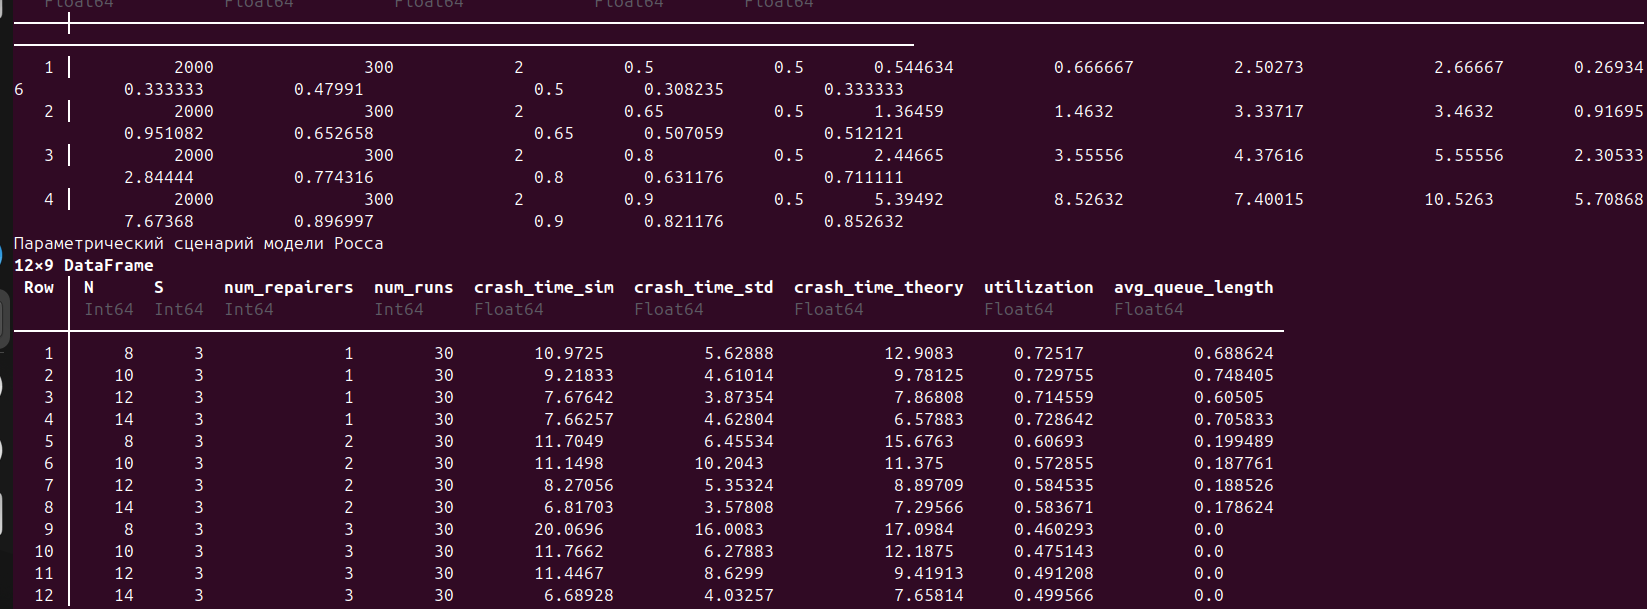
\includegraphics[width=1\linewidth,height=\textheight,keepaspectratio]{image/param_scenarios_table.png}
\end{column}

\begin{column}{0.5\linewidth}
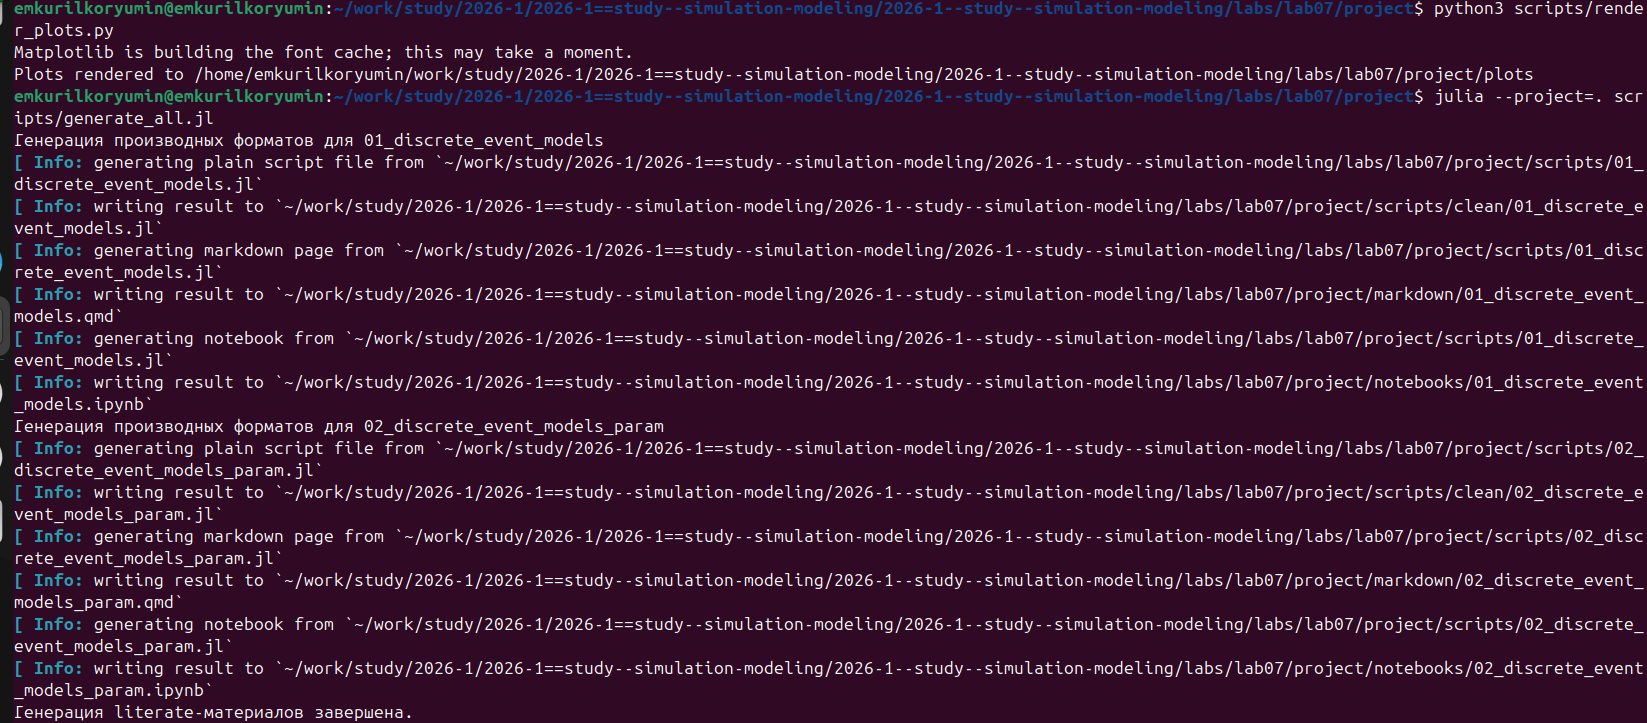
\includegraphics[width=1\linewidth,height=\textheight,keepaspectratio]{image/artifacts_generation_console.png}
\end{column}
\end{columns}

\begin{itemize}[<+->]
\tightlist
\item
  Слева: итоговая таблица параметрического исследования модели Росса
\item
  Справа: генерация графиков, \texttt{clean}, \texttt{qmd} и
  \texttt{ipynb}
\end{itemize}
\end{frame}

\section{Основные
выводы}\label{ux43eux441ux43dux43eux432ux43dux44bux435-ux432ux44bux432ux43eux434ux44b}

\begin{frame}[fragile]{Основные выводы}
\begin{itemize}[<+->]
\tightlist
\item
  Модель \texttt{M/M/c} воспроизводит ожидаемый рост ожидания при
  увеличении \texttt{λ}
\item
  Имитация \texttt{M/M/c} качественно согласуется с формулами Эрланга
  \texttt{C}
\item
  В модели Росса увеличение числа ремонтников повышает устойчивость
  системы
\item
  При росте числа машин увеличиваются загрузка ремонтников и очередь на
  ремонт
\item
  Имитационные оценки времени до отказа согласуются с аналитическим
  решением
\end{itemize}
\end{frame}




\end{document}
